\chapter{Hardware Design and Implementation}
\section{Concepts of DeAr}
\indent 
One of the key features of the proposed DeAr DSP is manipulating Simultaneous Multi-threading (SMT) in each lane with the purpose of exploiting arithmetic resources.
By scheduling two DeAr threads to collaborative execution, the workload of each work-item can be shared concurrently by two of them, 
which accelerate the execution of the wavefront and gain higher throughput without driving the clock speed or SIMD width.
Another feature is exhaustively compacting the hardware resources while keeping the flexibility and computation power.
This offers the DeAr DSP better efficiency in several perspectives including power consumption, chip area and memory usage.
\\\indent Figure~\ref{fig:basicblock:a} illustrate the typical execution flow of a work-item with several basic blocks, 
each of which refers to piece of code without any branch or jump instruction except its entry and exit.
The life cycle of a work-item involves processing basic blocks and migrating among them.
The acceleration is achieved by exploiting ILP in each basic block, as shown in Figure~\ref{fig:basicblock:b}. 
At the entry of a program, two DeAr threads are forked by the hardware in replacement of a work-item.
Next, the forked DeAr threads simultaneously fetch and execute the statically-scheduled instructions to exploit ILP within the basic block.
They join at the end of the basic block, and perform an identical branch or jump instruction targeting the next basic block simultaneously.
\section{Micro-architecture Design}
In this section, we will look into DeAr from a micro-architecture perspective, and explore its design considerations at the same time.
Figure~\ref{fig:micro} illustrates the micro-architecture of DeAr DSP lane.
We adopted the concept of Harvard architecture, 
which separates data memory and instruction memory physically\cite{harvard}.
As a result, the datapath and the control path are wrapped by two independent interfaces, the load/store unit and the instruction unit, respectively.
Such orthogonality between data and instructions offers better freedom of optimizing data precision or code density.
The load/store unit supports burst mode transfer, which enable consecutive fetch of the data in the memory.
This mechanism reduce the number of memory access instructions to be used, 
and improve the utilization of the bus bandwidth.
In addition, DeAr allows the memory transfer to be initiated by two threads orthogonally under the hardware arbitration.
On the other hand, since two DeAr threads always branch simultaneously to the same basic block, 
the compiler can align their simultaneous instructions to adjacent addresses.
As a result, the instruction unit can serve two DeAr threads by doubling the fetch width instead of duplication of the hardware.
\\\indent
Next, we are looking into the datapath.
Two DeAr threads in a lane not only share group of arithmetic units that commonly exist in a RISC datapath, 
but also the same instruction unit which is suitable for synchronous branch.
The demonstrated example includes an adder, a multiplier and a barrel shifter, which are qualified to perform most benchmarks,
Nevertheless, the configuration of arithmetic units can be modified to fit the target applications.
The output of each arithmetic unit is an accumulator register, 
which bypasses the result to any arithmetic units that need it in the next clock cycle.
The bypassing-mechanism of accumulator registers avoid unnecessary accesses to RF, 
and thus reduce the energy dissipation in RF.
In addition, the accumulator registers are all clock-gated.
This enables DeAr to preserve the data in accumulator registers until the corresponding arithmetic unit is activated next time, 
offering more data bypassing opportunities.
The bypassing mechanism and resolution of structural hazards are both handled by the software, 
so the hardware complexity of dynamic scheduling or bypassing units can be avoided or reduced.
\\\indent
The RF is physically and symmetrically divided for two DeAr threads.
Each of them owns a pair of queue memory as well as stack memory, 
and these memory units of two DeAr threads form the sequential-accessed banked RF.
The banked organization of the RF cuts off redundant connectivity among read/write ports and register cells.
Compared with the conventional centralized organization, 
the wire area, power consumption and access time of the banked organization are significantly improved, as discussed in Section~\ref{sec:rfcell}.
A queue pair, composed of a load-queue and a store-queue, 
serves as the buffer that connects the lower level of the memory hierarchy with the datapath.
A load-queue and a store-queues can be accessed from their both sides concurrently in the first-in-first-out (FIFO) fashion.
A DeAr thread reads input data from its load-queue and writes the result of computation to its store-queue, 
while the load/store unit accesses the queues in the opposite direction.
By preventing a queue from empty or full with clever scheduling, the latency of load/store via it can thus be hidden.
The stack memory, on the other hand, is responsible for the storage of intermediate data and load/store address.
The nature of a stack memory is last-in-first-out (LIFO), 
which is the key property of the DeAr scheduling algorithm (elaborated in Chapter~\ref{cha:software}).
Using the sequential-access memory rather than a random-access one in RF effectively reduces the length of control signal, 
since any access to the RF can be simplified to "PUSH" or "POP".
The reduction in the length of control signal gains high code density and save the wiring from the instruction unit to RF.
This is the key advantage of DeAr over conventional VLIW architectures.
For clarity, we summarize the classification of various data registers in the datapath in Table~\ref{tab:register}.
\begin{table}[!ht]
    \centering
    \begin{tabular}{|l|l|l|}
        \hline
        \multicolumn{1}{|c|}{\textbf{Register type}} & \multicolumn{1}{c|}{\textbf{Dedicated to}} & \multicolumn{1}{c|}{\textbf{Description}}                 \\ \hline
        Load-queue                                   & \multirow{3}{*}{a DeAr thread}             & buffers input data received from the main memory          \\ \cline{1-1} \cline{3-3} 
        Store-queue                                  &                                            & buffers output data sent to the main memroy               \\ \cline{1-1} \cline{3-3} 
        Stack                                        &                                            & buffers intermediate data of computation                  \\ \hline
        Accumulator                                  & an arithmetic unit                         & buffers the arithmetic result of the previous clock cycle \\ \hline
    \end{tabular}
    \caption{Classification of data registers in DeAr}
    \label{tab:register}
\end{table}
\\\indent
The compact data bus separates the RF and arithmetic units with a set of multiplexers controlled by the instruction unit.
The route of data over the compact data bus is summarized as below:
\begin{itemize}
    \item Each arithmetic unit receives the first operand from a load-queue or an accumulator.
        and receives the second one from a load-queue or a stack.
    \item Each store-queue receives data from the output of an arithmetic unit.
    \item Each stack receives data from the output of an arithmetic unit.
\end{itemize}
It is important to note that, even though the communication among the RF, arithmetic units and accumulator registers is compacted exhaustively, 
the flexibility of the datapath is still be kept.
By such a compact design of the data bus, the further reduction in the length of instrucions can be achieved.
More insight into the compact data bus will be available in Section~\ref{sec:isa}.

\vspace{\textfig}
\begin{figure}[!ht] 
    \centering
    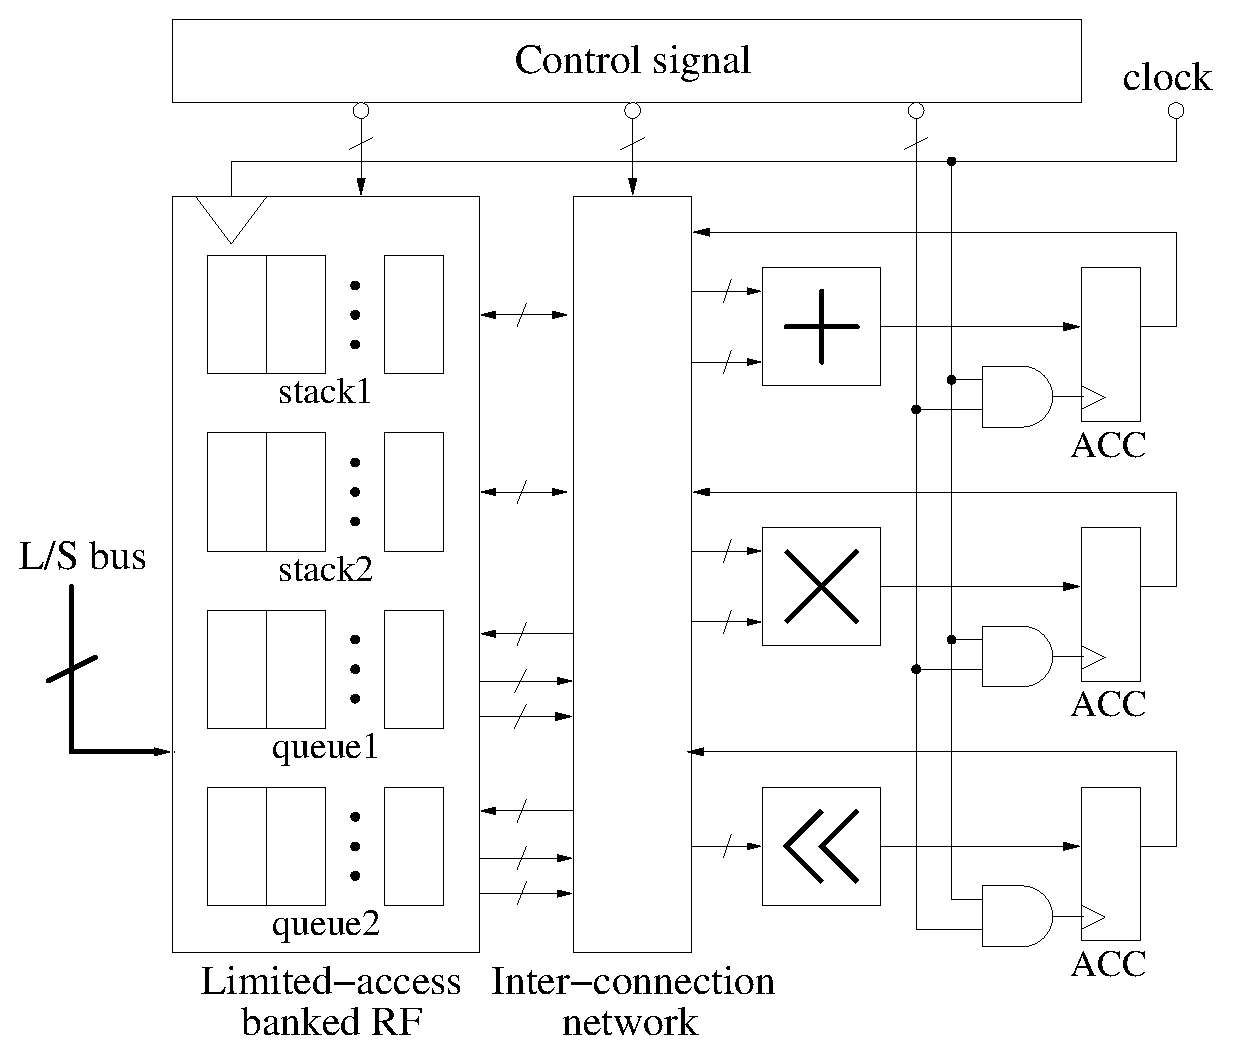
\includegraphics[width=0.85\textwidth]{./figs/micro.eps}
    \caption{Micro-architecture of a DeAr DSP lane}
    \label{fig:micro}
\end{figure}


\section{Instruction Set Architecture}
\label{sec:isa}
\indent The DeAr instruction set architecture (ISA) seemingly follows the principle of RISC, which takes instructions with fixed length, 
but the former is optimized for efficient arithmetic.
Each DeAr instruction is composed of two portions, RISC-style portion and stack-access portion.
The instruction unit issues two instructions simultaneously for two DeAr threads.
Table~\ref{tab:risc} shows the functions of the RISC-style portion, which are similar to some subset conventional RISC ISA.
Here, we use the bold alphabets, \textbf{b}, \textbf{s}, \textbf{t}, \textbf{k}, \textbf{a}, 
to represent the instruction decode bit-fields and illustrate the meaning of each function.
By considering their functions, they can be classified to three categories, A type, B type and M type.
A type includes arithmetic instructions such as addition (ADD or SUB), multiplication (MUL) and shift operation (SHL or SHR).
Other instructions like move (MV), which moves data from the other DeAr thread, 
and no operation (NOP), which stalls the DeAr thread for a cycle, 
belong to A type as well since they also manipulate arithmetic units.
B type includes instructions which interact with the instruction unit, such as branch on zero (BE) and branch on nonzero (BNE).
M type, on the other, includes memory transfer instructions, load (LD) and store (ST), which manage the load/store unit.
Any instruction must be followed by stack-access portion to form a complete DeAr instruction.
%---------- risc-style portion table
\begin{table}[ht!]
    \centering
    \begin{tabular}{|c|l|l|c|}
        \hline
        \multicolumn{1}{|c|}{\textbf{Category}} & \multicolumn{1}{c|}{\textbf{Name}} & \multicolumn{1}{c|}{\textbf{Meaning}} & \multicolumn{1}{c|}{\textbf{Target}} \\ \hline
        \multirow{7}{*}{ A type }      & ADD & \textbf{d} = \textbf{s} + \textbf{t}  & \multirow{7}{*}{Datapath}  \\ \cline{2-3}
                                       & SUB & \textbf{d} = \textbf{s} - \textbf{t} & \\ \cline{2-3} 
                                       & MUL & \textbf{d} = \textbf{s} * \textbf{t} & \\ \cline{2-3} 
                                       & SHL & \textbf{d} = \textbf{s} << \textbf{t} & \\ \cline{2-3}
                                       & SHR & \textbf{d} = \textbf{s} >> \textbf{t} & \\ \cline{2-3}
                                       & MV  & \textbf{d} = \textbf{s} + 0 or \textbf{d} = \textbf{s} << 0 & \\ \cline{2-3} 
                                       & NOP & \begin{tabular}[c]{@{}l@{}}1. disable write back \\ 2. clock-gate the accumulator \end{tabular}& \\ \hline
    \multirow{2}{*}{ B type }          & BZ  & \begin{tabular}[c]{@{}l@{}} \textit{if}{}\\ \ \ \ \ \ \ \ load\_queue.push (memory[\textbf{a}]) \end{tabular} & \multirow{2}{*}{Instruction unit} \\ \cline{2-3}
                                       & BNZ & conditional branch with the offset & \\ \hline
    \multirow{2}{*}{ M type}           & LD  & \begin{tabular}[c]{@{}l@{}} \textit{repeat}(\textbf{b})\\ \ \ \ \ \ \ \ load\_queue.push (memory[\textbf{a}]) \end{tabular}& \multirow{2}{*}{Load/store unit} \\ \cline{2-3} 
                                       & ST  & \begin{tabular}[c]{@{}l@{}} \textit{repeat}(\textbf{b})\\ \ \ \ \ \ \ \ memory[\textbf{a}] = store\_queue.pop() \end{tabular}& \\ \hline
    \end{tabular}
    \caption{RISC-style portion of the DeAr instruction set}
    \label{tab:risc}
\end{table}
%-----------------------------------------

\indent On the other hand, the stack-access portion, illustrated in Table~\ref{tab:stack}, 
is dedicated to manipulate the stack memory of the DeAr thread.
Four stack operations, PUSH, POP, MODIFY and NOP, are defined, 
Each DeAr thread uses these stack operations to buffer its intermediate results in the LIFO manner.
A PUSH operation stores the result from one of arithmetic units and adds the head address by 1, 
while a POP operation eliminate the head data by subtracting the head address by 1.
Since a POP operation followed by a PUSH operation modifies the data at the head data and maintains the head address, 
a MODIFY operation is defined to simplify the usage of two operations.
In some scenarios, the DeAr thread does nothing to the stack but keeps its condition.
As a result, a NOP operation is also defined for the stack-access portion.
Note that the NOP of stack-access portion should be distinguished from the one of RISC-style portion.
These two portions constitute DeAr ISA.
The DeAr thread can thus access an arithmetic units with the RISC-style protion and handle the intermediate result with stack-access portion.
On the other hand, since the memory transfer instrucions (i.e., LD and ST) never generate intermediate, 
they do not need the stack-access portion.
We can thus preserve more bits in the memory transfer instrucions to address larger memory space.

%---------- stack portion table
\begin{table}[ht!]
    \centering
    \begin{tabular}{|l|l|l|}
        \hline
        \multicolumn{1}{|c|}{\textbf{Name}} & \multicolumn{1}{c|}{\textbf{Meaning}} & \multicolumn{1}{c|}{\textbf{Note}} \\ \hline
    PUSH & \begin{tabular}[c]{@{}l@{}}1. Add the head address by 1\\ 2. Write the new data to the head address\end{tabular} & \multirow{2}{*}{ \parbox{5cm}{A "pop" followed by a "push" is equivalent to a "modify"} } \\ \cline{1-2}
    POP                               & \begin{tabular}[c]{@{}l@{}}1. Subtract the head address by 1\\ 2. Invalidate the previous head data\end{tabular} & \\ \hline
        MODIFY                            & Modify the head data to to the new data & The head address remains \\ \hline
        NOP                               & No operation & The head address and data remain \\ \hline
    \end{tabular}
    \caption{Stack access portion of the DeAr instrucion set}
    \label{tab:stack}
\end{table}
%-----------------------------------------

To offer an insight into the mechanism of DeAr instrucion decode, 
Table~\ref{tab:decode} elaborates each bit-filed of the instrucion, 
which correpsonds the bold alphabet in Table~\ref{tab:risc}.
Note that this table reveals the details of the compact data bus of Figure~\ref{fig:micro}, 
since the former also elaborates the data communication via the latter.
For the category of non-memory transfer, there are six bit-fields in each instrucion.
We will enumerate each bit-field from MSB to LSB of the instrucion.
The MSB, \textbf{m}, indicates which category (memory transfer or non-memory transfer) this instrucion belongs to.
The 3-bit signal, \textbf{f}, which is similar to the operation code in RISC, specifies the operation to be performed.
Another single-bit signal, \textbf{d}, determines whether the result of this operaion is written back to the memory via the store-queue.
A pair of 2-bit signals, \textbf{s} and \textbf{t}, select the sources of two arithmetic operands respectively. 
Nevertheless, their potential sources are not identical.
The former select the first operand from the load-queue or one of accumulator registers, 
while the later select the second one from the load-queue, stack, or constants.
The last bit-field of non-memory transfer instrucion, \textbf{k}, encodes four operations that manipulate the stack memroy with 2 bits.
Each of stack-access operations is elaborated in Table~\ref{tab:stack}.
\\\indent On the other hand, a memory transfer instrucion only includes three bit-fields.
The funcion of MSB, \textbf{m}, is identical to the one of a non-memory transfer instrucion, 
but its value is fixed to one to idicate the request for memory transfer.
The following bit, \textbf{l}, specifies the direction this memory transfer.
The last bit-field of the rest of bits, \textbf{a}, determines the data address of this memory transer in the main memory.
%---------- bit field table---------------
\begin{table}[!ht]
    \centering
    \begin{tabular}{|l|l|l|}
        \hline
        \multicolumn{1}{|c|}{\textbf{Mark}} & \multicolumn{1}{c|}{\textbf{Bit field [10:0]}} & \multicolumn{1}{c|}{\textbf{Description}} \\ \hline
        \multicolumn{3}{|c|}{\textbf{Non-memory transfer instructions}} \\ \hline
        m & {[}10{]} & This bit is fixed to 0 for non-memory transfer instructions \\ \hline
    f & {[}9:7{]} & \begin{tabular}[c]{@{}l@{}}Specify the function of this instruction, which can be\\ ADD, SUB, SHL, SHR, MUL, MV or NOP\end{tabular} \\ \hline
    d & {[}6{]} & \begin{tabular}[c]{@{}l@{}}Specify that the arithmetic result will be write back to \\ the store-queue\end{tabular} \\ \hline
    s & {[}5:4{]} & \begin{tabular}[c]{@{}l@{}}Specify the source of the first arithmetic operand, \\ which can be the load-queue or one of accumulators\end{tabular} \\ \hline
    t & {[}3:2{]} & \begin{tabular}[c]{@{}l@{}}Specify the source of the second arithmetic operand, \\ which can be the load-queue, stack, constant 0 or 1\end{tabular} \\ \hline
    k & {[}1:0{]} & \begin{tabular}[c]{@{}l@{}}Specify the stack operation, which can be PUSH, POP, \\ MODIFY or NOP (stack access portion)\end{tabular} \\ \hline
        \multicolumn{3}{|c|}{\textbf{Memory transfer instruction}} \\ \hline
        m & {[}10{]} & This bit is fixed to 1 for memory transfer instructions \\ \hline
        l & {[}9{]} & Specify the transfer type, which can be LD or ST\\ \hline
        a & {[}8:0{]} & Specify the address of the transfer \\ \hline
    \end{tabular}
    \caption{Instrucion decode table of the DeAr instrucion set}
    \label{tab:decode}
\end{table}
%------------------------------------------

\section{System Integration}
